\documentclass[landscape,a0paper,fontscale=0.292]{baposter}

\usepackage{times}
\usepackage{calc}
\usepackage{url}
\usepackage{graphicx}
\usepackage{amsmath}
\usepackage{amssymb}
\usepackage{relsize}
\usepackage{multirow}
\usepackage{booktabs}

\usepackage{graphicx}
\usepackage{multicol}
\usepackage[T1]{fontenc}
\usepackage{ae}

\graphicspath{{images/}}

 %%%%%%%%%%%%%%%%%%%%%%%%%%%%%%%%%%%%%%%%%%%%%%%%%%%%%%%%%%%%%%%%%%%%%%%%%%%%%%%%
 %%%% Some math symbols used in the text
 %%%%%%%%%%%%%%%%%%%%%%%%%%%%%%%%%%%%%%%%%%%%%%%%%%%%%%%%%%%%%%%%%%%%%%%%%%%%%%%%
 % Format 
 \newcommand{\RotUP}[1]{\begin{sideways}#1\end{sideways}}


 %%%%%%%%%%%%%%%%%%%%%%%%%%%%%%%%%%%%%%%%%%%%%%%%%%%%%%%%%%%%%%%%%%%%%%%%%%%%%%%%
 % Multicol Settings
 %%%%%%%%%%%%%%%%%%%%%%%%%%%%%%%%%%%%%%%%%%%%%%%%%%%%%%%%%%%%%%%%%%%%%%%%%%%%%%%%
 \setlength{\columnsep}{0.7em}
 \setlength{\columnseprule}{0mm}


 %%%%%%%%%%%%%%%%%%%%%%%%%%%%%%%%%%%%%%%%%%%%%%%%%%%%%%%%%%%%%%%%%%%%%%%%%%%%%%%%
 % Save space in lists. Use this after the opening of the list
 %%%%%%%%%%%%%%%%%%%%%%%%%%%%%%%%%%%%%%%%%%%%%%%%%%%%%%%%%%%%%%%%%%%%%%%%%%%%%%%%
 \newcommand{\compresslist}{%
 \setlength{\itemsep}{1pt}%
 \setlength{\parskip}{0pt}%
 \setlength{\parsep}{0pt}%
 }


 %%%%%%%%%%%%%%%%%%%%%%%%%%%%%%%%%%%%%%%%%%%%%%%%%%%%%%%%%%%%%%%%%%%%%%%%%%%%%%
 % Formating
 \newcommand{\Matrix}[1]{\begin{bmatrix} #1 \end{bmatrix}}
 \newcommand{\Vector}[1]{\begin{pmatrix} #1 \end{pmatrix}}

 \newcommand*{\norm}[1]{\mathopen\| #1 \mathclose\|}% use instead of $\|x\|$
 \newcommand*{\abs}[1]{\mathopen| #1 \mathclose|}% use instead of $\|x\|$
 \newcommand*{\normLR}[1]{\left\| #1 \right\|}% use instead of $\|x\|$

 \newcommand*{\SET}[1]  {\ensuremath{\mathcal{#1}}}
 \newcommand*{\FUN}[1]  {\ensuremath{\mathcal{#1}}}
 \newcommand*{\MAT}[1]  {\ensuremath{\boldsymbol{#1}}}
 \newcommand*{\VEC}[1]  {\ensuremath{\boldsymbol{#1}}}
 \newcommand*{\CONST}[1]{\ensuremath{\mathit{#1}}}

 \DeclareMathOperator*{\argmax}{arg\,max}
 \DeclareMathOperator*{\diag}{diag}
 \DeclareMathOperator*{\argmin}{arg\,min}
 \DeclareMathOperator*{\vectorize}{vec}
 \newcommand{\vect}[1]{\boldsymbol{#1}}  % bm alternative
 \DeclareMathOperator*{\reshape}{reshape}

 %-----------------------------------------------------------------------------
 % Differentiation
 \newcommand*{\Nabla}[1]{\nabla_{\!#1}}

 \renewcommand*{\d}{\mathrm{d}}
 \newcommand*{\dd}{\partial}

 \newcommand*{\At}[2]{\ensuremath{\left.#1\right|_{#2}}}
 \newcommand*{\AtZero}[1]{\At{#1}{\pp=\VEC 0}}

 \newcommand*{\diffp}[2]{\ensuremath{\frac{\dd #1}{\dd #2}}}
 \newcommand*{\diffpp}[3]{\ensuremath{\frac{\dd^2 #1}{\dd #2 \dd #3}}}
 \newcommand*{\diffppp}[4]{\ensuremath{\frac{\dd^3 #1}{\dd #2 \dd #3 \dd #4}}}
 \newcommand*{\difff}[2]{\ensuremath{\frac{\d #1}{\d #2}}}
 \newcommand*{\diffff}[3]{\ensuremath{\frac{\d^2 #1}{\d #2 \d #3}}}
 \newcommand*{\difffp}[3]{\ensuremath{\frac{\dd\d #1}{\d #2 \dd #3}}}
 \newcommand*{\difffpp}[4]{\ensuremath{\frac{\dd^2\d #1}{\d #2 \dd #3 \dd #4}}}

 \newcommand*{\diffpAtZero}[2]{\ensuremath{\AtZero{\diffp{#1}{#2}}}}
 \newcommand*{\diffppAtZero}[3]{\ensuremath{\AtZero{\diffpp{#1}{#2}{#3}}}}
 \newcommand*{\difffAt}[3]{\ensuremath{\At{\difff{#1}{#2}}{#3}}}
 \newcommand*{\difffAtZero}[2]{\ensuremath{\AtZero{\difff{#1}{#2}}}}
 \newcommand*{\difffpAtZero}[3]{\ensuremath{\AtZero{\difffp{#1}{#2}{#3}}}}
 \newcommand*{\difffppAtZero}[4]{\ensuremath{\AtZero{\difffpp{#1}{#2}{#3}{#4}}}}

 %-----------------------------------------------------------------------------
 % Defined
 % How should the defined operator look like (:= or ^= ==)
 % (I want back my :=, it is so much better than ^= because (1) it has a
 % direction and (2) everyone here uses it.)
 %
 % Use :=
 %\newcommand*{\defined}{\ensuremath{\mathrel{\mathop{:}}=}}
 %\newcommand*{\definedRight}{\ensuremath{=\mathrel{\mathop{:}}}}
 % Use ^=
 \newcommand*{\defined}{\ensuremath{\triangleq}}
 \newcommand*{\definedRight}{\ensuremath{\triangleq}}
 % Use = with three bars
 %\newcommand*{\defined}{\ensuremath{?}}
 %\newcommand*{\definedRight}{\ensuremath{?}}

 %%%%%%%%%%%%%%%%%%%%%%%%%%%%%%%%%%%%%%%%%%%%%%%%%%%%%%%%%%%%%%%%%%%%%%%%%%%%%%
 % Symbols used in the paper

 %-----------------------------------------------------------------------------
 % The Methods
 \newcommand*{\ICIA}{\emph{ICIA}}
 \newcommand*{\CoDe}{\emph{CoDe}}
 \newcommand*{\LinCoDe}{\emph{LinCoDe}}
 \newcommand*{\CoNe}{\emph{CoNe}}
 \newcommand*{\CoLiNe}{\emph{CoLiNe}}
 \newcommand*{\LinCoLiNe}{\emph{LinCoLiNe}}

 % inter eye distance
 \newcommand*{\ied}{IED}

 %-----------------------------------------------------------------------------
 % Koerper
 %%\newcommand*{\RR}{\mathbb{R}}
 %\newcommand*{\RR}{{I\hspace{-3.5pt}R}}
 %\newcommand*{\RR}{{\mathrm{I\hspace{-2.7pt}R}}}

 \font\dsfnt=dsrom12

 \DeclareSymbolFont{nark}{U}{dsrom}{m}{n}
 \DeclareMathSymbol{\NN}{\dsfnt}{nark}{`N}
 \DeclareMathSymbol{\RR}{\dsfnt}{nark}{`R}
 \DeclareMathSymbol{\ZZ}{\dsfnt}{nark}{`Z}

 %-----------------------------------------------------------------------------
 % Domains
 \newcommand*{\D}{\mathcal{D}}
 \newcommand*{\I}{\mathcal{I}}

 %-----------------------------------------------------------------------------
 % Texture coordinates
 \newcommand*{\rr}{\VEC{r}}

 %-----------------------------------------------------------------------------
 % Parameters
 \newcommand*{\pt}{\VEC{\tau}}
 \newcommand*{\pr}{\VEC{\rho}}
 \newcommand*{\pp}{\VEC{p}}
 \newcommand*{\qq}{\VEC{q}}
 \newcommand*{\xx}{\VEC{x}}
 \newcommand*{\deltaq}{\Delta \qq}
 \newcommand*{\deltap}{\Delta \pp}
 \newcommand*{\zz}{\VEC{z}}
 \newcommand*{\pa}{\VEC{\alpha}}
 \newcommand*{\qa}{\VEC{\alpha}}
 \newcommand*{\pb}{\VEC{\beta}}

 %-----------------------------------------------------------------------------
 % Optimal appearance parameters
 \newcommand*{\pbh}[1]{\ensuremath{\hat{\pb}({#1})}}

 %-----------------------------------------------------------------------------
 % Warp basis
 \newcommand*{\M}[1]{\ensuremath{M({#1})}}
 \newcommand*{\LL}[1]{\ensuremath{L({#1})}}

 %-----------------------------------------------------------------------------
 % Matrices of the texture model
 \newcommand*{\AM}[1]{\ensuremath{\Lambda(#1)}}               % Lambda(beta) 
 \newcommand*{\AMr}[2]{\ensuremath{\Lambda(#1; #2)}}        % Lambda(r, beta)

 \newcommand*{\As}{A}         % Continuous Basis symbol
 \newcommand*{\afs}{a}        % Continuous mean symbol
 \newcommand*{\A}[1]{\As(#1)}         % Continuous Basis
 \newcommand*{\af}[1]{\afs(#1)}        % Continuous mean


 %-----------------------------------------------------------------------------
 % Matrices of the shape model
 \newcommand*{\MU}{\VEC{\mu}}
 \newcommand*{\MM}{\MAT{M}}

 %-----------------------------------------------------------------------------
 %% The project out matrix and operator
 \newcommand*{\INT}{\MAT{P}}
 \newcommand*{\INTf}{P}

 %-----------------------------------------------------------------------------
 % The identity matrix
 \newcommand*{\EYEtwo}{\Matrix{1 & 0\\0&1}}
 \newcommand*{\EYE}{\MAT E}
 \newcommand*{\EYEf}{E}

 % Wether to use subscripts or brackets for some function arguments
 % can be decided by commenting out the corresponding functions underneath
 %-----------------------------------------------------------------------------
 % Mapping
 \newcommand*{\Cs}[1]{\ensuremath{C^{#1}}} % C symbol
 \newcommand*{\C}[2]{\ensuremath{C^{#1}(#2)}} % Use C with brackets

 %-----------------------------------------------------------------------------
 % Objective function
 \newcommand*{\Fs}{\ensuremath{F}}              % F symbol
 \newcommand*{\F}[1]{\ensuremath{\Fs(#1)}}       % Use F with brackets    F(q)

 %-----------------------------------------------------------------------------
 % Approximated objective functions
 \newcommand*{\FFs}{\tilde{F}}                     % ~F symbol
 \newcommand*{\FF}[1]{\ensuremath{\FFs(#1)}}       % Use ~F with brackets    F(q)

 %-----------------------------------------------------------------------------
 % residual function
 \newcommand*{\es}{\ensuremath{f}}              % R symbol

 \newcommand*{\e}[1]{\ensuremath{\es(#1)}}         % R(q)
 \newcommand*{\er}[2]{\ensuremath{\es(#1; #2)}}    % R(r; q)

 %-----------------------------------------------------------------------------
 % Approximated residual functions
 \newcommand*{\ees}{\tilde{f}}                       % ~R symbol
 \newcommand*{\ee}[1]{\ensuremath{\ees(#1)}}       % ~R(q)
 \newcommand*{\eer}[2]{\ensuremath{\ees(#2; #1)}}  % ~R(r; q)

 %-----------------------------------------------------------------------------
 % Warps
 \newcommand*{\Vs}{\ensuremath{V}}
 \newcommand*{\VLins}{\ensuremath{\Vs^{\text{Ortho}}}}
 \newcommand{\VModels}{\ensuremath{\Vs^{\text{Model}}}}
 \newcommand*{\Ws}{\ensuremath{W}}

 \newcommand{\V}[1]{\ensuremath{\Vs(#1)}}
 \newcommand{\VModel}[1]{\ensuremath{\VModels(#1)}}
 \newcommand{\Vr}[2]{\ensuremath{\Vs(#1; #2)}}
 \newcommand{\VInvr}[2]{\ensuremath{\Vs^{-1}(#1; #2)}}
 \newcommand{\VrLin}[2]{\ensuremath{\VLins(#1; #2)}}
 \newcommand{\W}[1]{\ensuremath{\Ws(#1)}}
 \newcommand{\Winv}[1]{\ensuremath{\Ws^{-1}(#1)}}
 \newcommand{\Wr}[2]{\ensuremath{\Ws(#1; #2)}}
 
 % Shortnames
 \newcommand{\etal}{\textit{et al}. }


%%%%%%%%%%%%%%%%%%%%%%%%%%%%%%%%%%%%%%%%%%%%%%%%%%%%%%%%%%%%%%%%%%%%%%%%%%%%%
%% Begin of Document
%%%%%%%%%%%%%%%%%%%%%%%%%%%%%%%%%%%%%%%%%%%%%%%%%%%%%%%%%%%%%%%%%%%%%%%%%%%%%
\begin{document}
%%%%%%%%%%%%%%%%%%%%%%%%%%%%%%%%%%%%%%%%%%%%%%%%%%%%%%%%%%%%%%%%%%%%%%%%%%%%%
%% Here starts the poster
%%---------------------------------------------------------------------------
%% Format it to your taste with the options
%%%%%%%%%%%%%%%%%%%%%%%%%%%%%%%%%%%%%%%%%%%%%%%%%%%%%%%%%%%%%%%%%%%%%%%%%%%%%
\begin{poster}{
 % Show grid to help with alignment
 grid=false,
 % Column spacing
 colspacing=0.7em,
 % Color style
 headerColorOne=cyan!20!white!90!black,
 borderColor=cyan!30!white!90!black,
 % Format of textbox
 textborder=faded,
 % Format of text header
 headerborder=open,
 headershape=roundedright,
 headershade=plain,
 background=none,
 bgColorOne=cyan!10!white,
 headerheight=0.16\textheight}
 % Eye Catcher
 {
%      \includegraphics[width=0.08\linewidth]{track_frame_00010_06}
%      \includegraphics[width=0.08\linewidth]{track_frame_00450_06}
%      \includegraphics[width=0.08\linewidth]{track_frame_04999_06}
 }
 % Title
 {DDRNet: Depth Map Denoising and Refinement for Consumer Depth Cameras Using Cascaded CNNs}
 % Authors
 {Shi Yan$^1$, Chenglei Wu$^2$,	Lizhen Wang$^1$, Feng Xu$^1$, Liang An$^1$, Kaiwen Guo$^3$ and Yebin Liu$^1$\\
 {$^1$Tsinghua University, $^2$Facebook Reality Labs, $^3$Google Inc}}
 % University logo
 {
  \begin{tabular}{c}
    
\includegraphics[height=0.12\textheight]{thu-fig-logo.pdf}\\
%    \raisebox{0em}[0em][0em]{\includegraphics[height=0.03\textheight]{msrlogo}}
  \end{tabular}
 }

%%%%%%%%%%%%%%%%%%%%%%%%%%%%%%%%%%%%%%%%%%%%%%%%%%%%%%%%%%%%%%%%%%%%%%%%%%%%%%
%%% Now define the boxes that make up the poster
%%%---------------------------------------------------------------------------
%%% Each box has a name and can be placed absolutely or relatively.
%%% The only inconvenience is that you can only specify a relative position 
%%% towards an already declared box. So if you have a box attached to the 
%%% bottom, one to the top and a third one which should be inbetween, you 
%%% have to specify the top and bottom boxes before you specify the middle 
%%% box.
%%%%%%%%%%%%%%%%%%%%%%%%%%%%%%%%%%%%%%%%%%%%%%%%%%%%%%%%%%%%%%%%%%%%%%%%%%%%%%

%%%%%%%%%%%%%%%%%%%%%%%%%%%%%%%%%%%%%%%%%%%%%%%%%%%%%%%%%%%%%%%%%%%%%%%%%%%%%%
  \headerbox{Motivation}{name=introduction,column=0,row=0,span=1}{
%%%%%%%%%%%%%%%%%%%%%%%%%%%%%%%%%%%%%%%%%%%%%%%%%%%%%%%%%%%%%%%%%%%%%%%%%%%%%%
  Consumer depth sensors suffer from heavy noises which limit their applications.
  Neural networks are capable of modeling complex functions and meet the real-time requirement. By leveraging single frame depth map and the accompanying high quality color image through a joint training strategy, we can achieve enhanced depth map.
  }
%%%%%%%%%%%%%%%%%%%%%%%%%%%%%%%%%%%%%%%%%%%%%%%%%%%%%%%%%%%%%%%%%%%%%%%%%%%%%%
\headerbox{Challenge}{name=Problems,column=1,row=0,span=1}{
	%%%%%%%%%%%%%%%%%%%%%%%%%%%%%%%%%%%%%%%%%%%%%%%%%%%%%%%%%%%%%%%%%%%%%%%%%%%%%%
	
	The challenge is to generate details and keep depth merically accurate. To lift the depth quality in low frequency and high frequency simultaneously, we propose a cascaded CNN structure to perform depth image denoising and refinement. To transfer surface details, we design a generative process together with an unsupervised loss based on rendering equation.
	% To go beyond training data
}
%%%%%%%%%%%%%%%%%%%%%%%%%%%%%%%%%%%%%%%%%%%%%%%%%%%%%%%%%%%%%%%%%%%%%%%%%%%%%%
  \headerbox{Pipeline \emph{and} Dataset}{name=pipeline,column=0,span=2,below=introduction}{
%%%%%%%%%%%%%%%%%%%%%%%%%%%%%%%%%%%%%%%%%%%%%%%%%%%%%%%%%%%%%%%%%%%%%%%%%%%%%%
	\begin{minipage}{0.67\linewidth}
		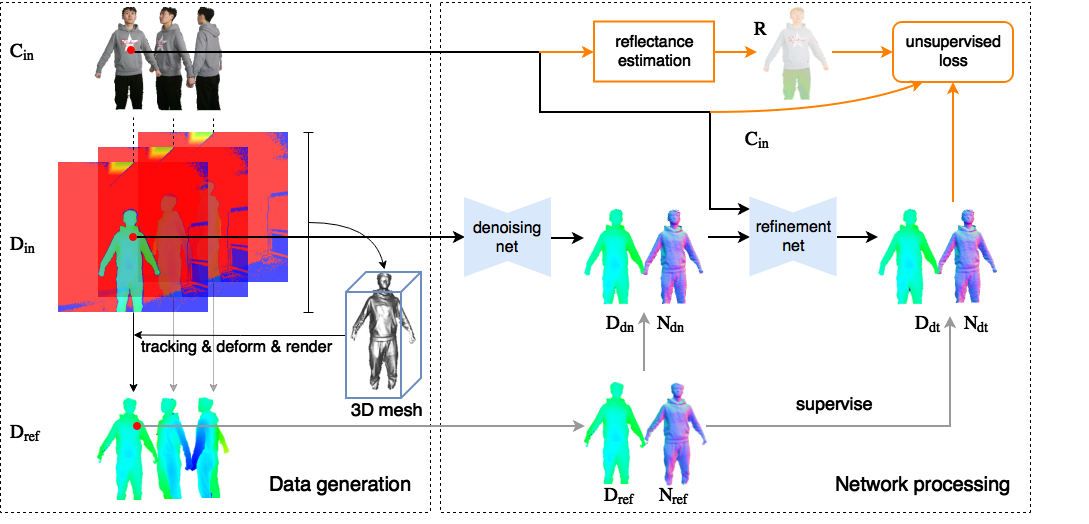
\includegraphics[width=\linewidth]{pipe.png}
	\end{minipage}\hfill
	\begin{minipage}{0.33\linewidth}
		The proposed pipeline features our novelties in training
		data creation and cascaded archietecture design.
		
		\textbf{Unlike synthesized data}, to capture noise pattern from real scenes, we employ multi-frame depth fusion technique to generate data.
		
		\textbf{We formulate the problem} into two regression tasks specific in different frequency domains. The cascaded CNNs learn from supervised depth data and unsupervised shading cues in an end-to-end way.
	\end{minipage}\hfill
}

 %%%%%%%%%%%%%%%%%%%%%%%%%%%%%%%%%%%%%%%%%%%%%%%%%%%%%%%%%%%%%%%%%%%%%%%%%%%%%%
   \headerbox{Denoising Method}{name=denoise,column=2,row=0,span=1}{
 %%%%%%%%%%%%%%%%%%%%%%%%%%%%%%%%%%%%%%%%%%%%%%%%%%%%%%%%%%%%%%%%%%%%%%%%%%%%%%
 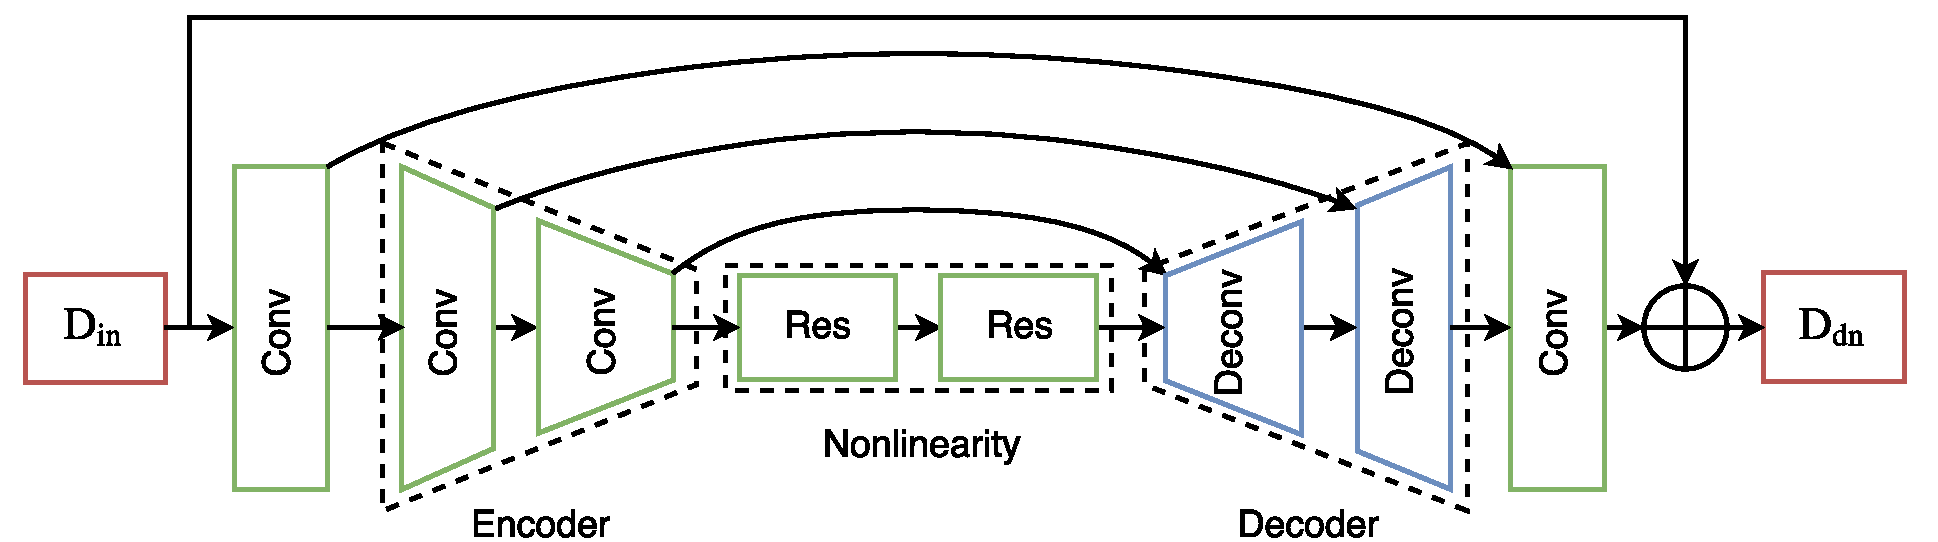
\includegraphics[width=\linewidth]{dnnet.pdf}
 \textbf{Fig. 2.} The structure of our denoising net. We adopt residual learning strategy to initialize denoising net and resolve vanishing gradients.
 
 \textbf{Loss} consists of 2 parts, reconstruction term constrains depth and normaldot term constrains normal direction, which remove noise in local patch.
 \begin{align}
 &\ell_{rec} (D_{dn}, D_{ref})\! =\! \lVert D_{dn}-D_{ref} \lVert_1\! + \! \lVert D_{dn} - D_{ref} \lVert_2 \notag \\
 &\ell_{dot} (D_{dn}, N_{ref}) \!=\! \sum_i \!\sum_{j \in {\mathcal N(i)}} \left[ <P^i-P^j, N_{ref}^i> \right]^2 \notag \\
 &{\mathcal L}_{dn}(D_{dn}, D_{ref}) = \lambda_{rec} \ell_{rec} + \lambda_{dot} \ell_{dot} \notag
 \end{align}
}

 %%%%%%%%%%%%%%%%%%%%%%%%%%%%%%%%%%%%%%%%%%%%%%%%%%%%%%%%%%%%%%%%%%%%%%%%%%%%%%
   \headerbox{Refinement Method}{name=refine,column=3,row=0,span=1}{
 %%%%%%%%%%%%%%%%%%%%%%%%%%%%%%%%%%%%%%%%%%%%%%%%%%%%%%%%%%%%%%%%%%%%%%%%%%%%%%
   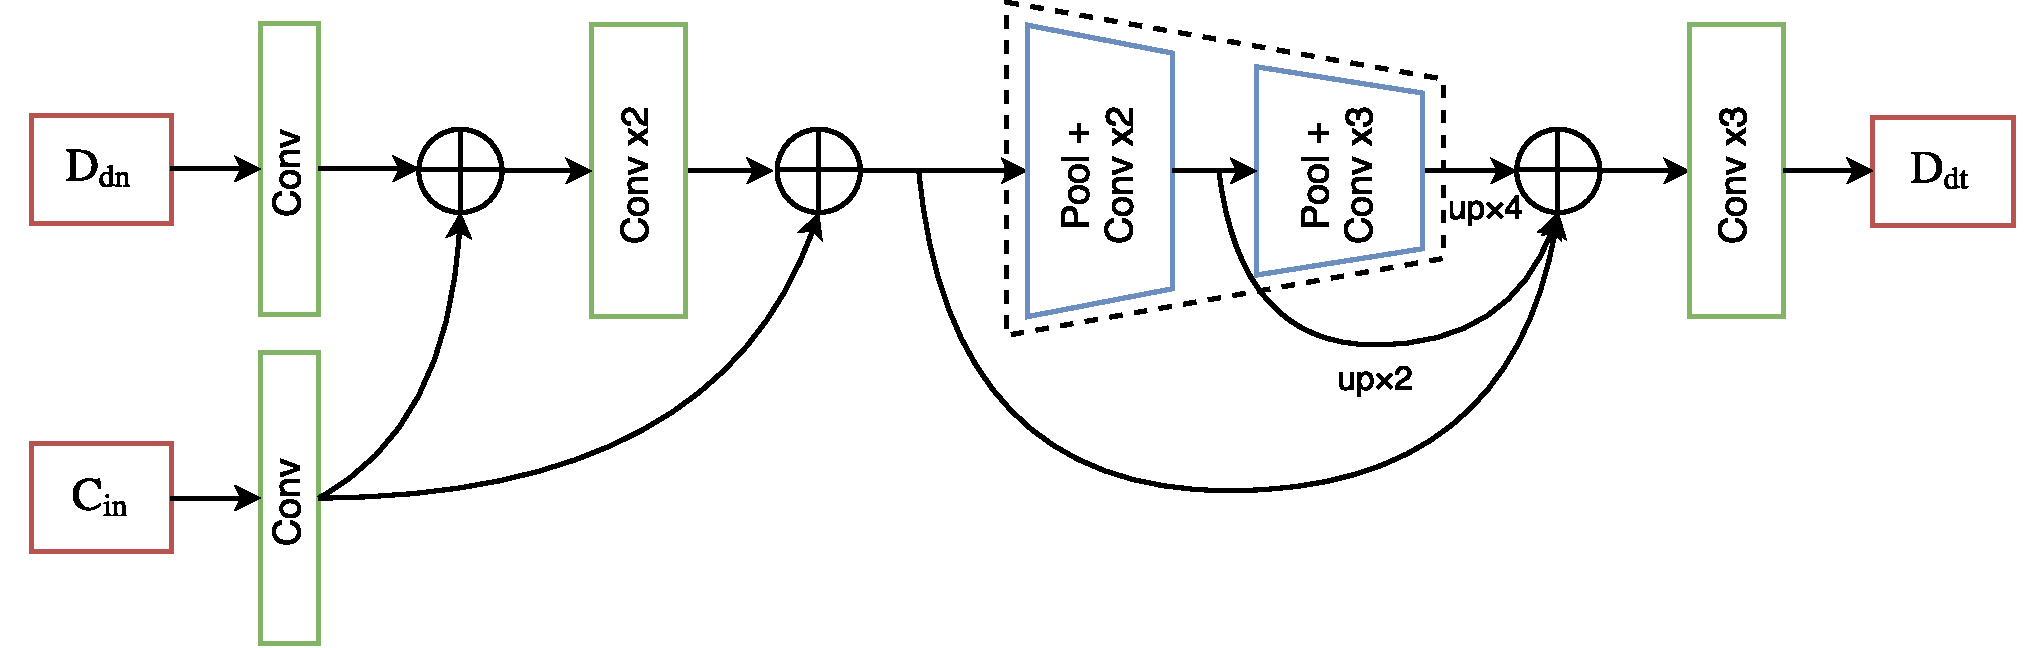
\includegraphics[width=\linewidth]{dtnet.pdf}
   \textbf{Fig. 3.} Refinement net structure. The convolved feature maps from depth map are complemented with the corresponding feature maps from RGB.
   
   \textbf{Reflected Irradiance} is a function of normal, lighting and albedo. $B(\vect{l}, N, R) = R \sum_{b=1}^9 l_b H_b(N)$
   
   \textbf{Light} coefficients are computed by solving least square problem. Albedos are estimated from RGB.

   \textbf{Loss} consists of 2 parts, shading term extrudes surface details and fidelity term keeps depth faithful.
   \vspace{-2em}
   \begin{align}
   \ell_{sh} (N_{dt}, N_{ref}, I) = &\lVert B(\vect{l}^*, N_{dt}, R) -  I \lVert_2  \notag \\
    &+ \lambda_{g} \lVert \nabla B(\vect{l}^*, N_{dt}, R) - \nabla I \lVert_2 \notag \\
   \ell_{fid}(D_{dt}, D_{ref}) = &\lVert D_{dt} - D_{ref} \lVert_2 \notag
   \end{align}
  }


% %%%%%%%%%%%%%%%%%%%%%%%%%%%%%%%%%%%%%%%%%%%%%%%%%%%%%%%%%%%%%%%%%%%%%%%%%%%%%%
%   \headerbox{References}{name=references,column=0,above=bottom}{
% %%%%%%%%%%%%%%%%%%%%%%%%%%%%%%%%%%%%%%%%%%%%%%%%%%%%%%%%%%%%%%%%%%%%%%%%%%%%%%
%     \smaller
%     
%     \bibliographystyle{ieee}
%     \renewcommand{\section}[2]{\vskip 0.05em}
%       \begin{thebibliography}{1}\itemsep=-0.01em
%       \setlength{\baselineskip}{0.4em}
%
%       \bibitem{amberg07:nicp}
%       B.~Amberg, A.~Blake, T.~Vetter
%       \newblock On Compositional Image Alignment with an Application to Activce Appearance Models
%       \newblock In {\em CVPR'09}, 2009.
%
%       \end{thebibliography}
%   }

 %%%%%%%%%%%%%%%%%%%%%%%%%%%%%%%%%%%%%%%%%%%%%%%%%%%%%%%%%%%%%%%%%%%%%%%%%%%%%%

 %%%%%%%%%%%%%%%%%%%%%%%%%%%%%%%%%%%%%%%%%%%%%%%%%%%%%%%%%%%%%%%%%%%%%%%%%%%%%%
\headerbox{Qualitative Result}{name=qualitative,column=0,span=2,below=pipeline}{
	%%%%%%%%%%%%%%%%%%%%%%%%%%%%%%%%%%%%%%%%%%%%%%%%%%%%%%%%%%%%%%%%%%%%%%%%%%%%%%
	\centering
	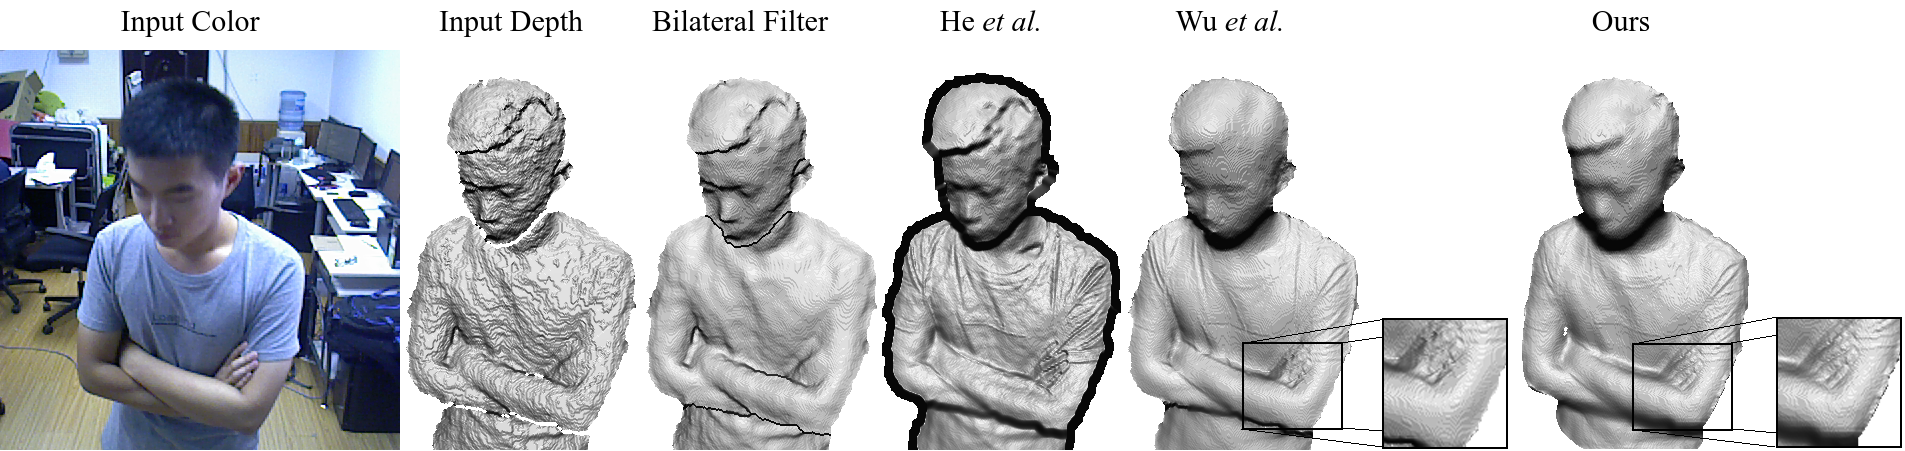
\includegraphics[width=\linewidth]{contrast.png}
	
	\textbf{Fig. 1.} Comparison of color-assisted depth map enhancement between bilateral filter, He \etal, Wu \etal and our method. The closeup of the finger demonstrates the effectiveness of unsupervised shading term.
	%in our refinement net loss.
}

   \headerbox{Quantitative Result}{name=quantitative,column=2,span=2,below=refine}{
 %%%%%%%%%%%%%%%%%%%%%%%%%%%%%%%%%%%%%%%%%%%%%%%%%%%%%%%%%%%%%%%%%%%%%%%%%%%%%%
 {
 	\begin{center}
 		\textbf{Table 1.} Average score of depth and normal error and on our ToF validation set.
 	\end{center}
	\vspace{-0.5em}
	\begin{tabular}{l|ccccc|ccccc}
	\hline
	\multirow{2}{*}{Method} & \multicolumn{5}{c|}{Depth difference}   & \multicolumn{5}{c}{Normal difference}         \\ \cline{2-11} 
	& seq. 1         & seq. 2         & seq. 3         & seq. 4         & seq. 5         & Mean $\downarrow$  & Median $\downarrow$ & 3.0$\uparrow$   & 5.0$\uparrow$   & 10.0$\uparrow$     \\ \hline
	Wu \etal    & 27.60          & 22.19          & 21.34          & 22.41          & 25.67          & 11.20         & 5.02          & 29.81          & 50.24          & 76.62          \\ \hline
	Or-El \etal    & 27.14          & 25.42          & 22.89          & 21.31          & 26.08          & 10.03         & 4.12          & 35.43          & 56.57          & 79.99          \\ \hline
	Ours  $ D_{dn} $    & 19.03          & \textbf{19.25} & 18.49          & \textbf{18.37} & 18.76          & \textbf{9.36} & \textbf{3.40} & \textbf{45.33} & \textbf{66.79} & \textbf{84.69} \\ \hline
	Ours  $ D_{dt} $    & \textbf{18.97} & 19.41          & \textbf{18.38} & 18.50          & \textbf{18.61} & 9.55          & 3.54          & 43.77          & 64.98          & 83.69          \\ \hline
 	\end{tabular}
 }

   \vspace{0.5em}
	The ground truth 3D model is obtained from laser scanner. After reprojection, rescaling and ICP, RMSE and MAE are calculated for depth map. We also report
	the angular difference of normals in degree.
%   \begin{multicols}{2}
%   \textbf{Our algorithm makes fast and robust tracking possible.}
%   The same training dataset was used for both tracking experiments. The
%   training data was aquired with different camera and light settings from
%   different subjects.
%   \end{multicols}
  }

 %%%%%%%%%%%%%%%%%%%%%%%%%%%%%%%%%%%%%%%%%%%%%%%%%%%%%%%%%%%%%%%%%%%%%%%%%%%%%%
\headerbox{Implementation Details}{name=implement,column=2,below=quantitative}{
	%%%%%%%%%%%%%%%%%%%%%%%%%%%%%%%%%%%%%%%%%%%%%%%%%%%%%%%%%%%%%%%%%%%%%%%%%%%%%%
Our training set contains 11540 views of structured light data and 25300 views of time-of-flight data.To adapt to different intrinsic parameters, we augment the intrinsic matrix and its 2.5D depth map accordingly. The forward pass takes only 20.4ms for 640 $\times$ 480 input on TitanX.
Get the model and code at: \mbox{\url{github.com/neycyanshi/DDRNet}}
}

 %%%%%%%%%%%%%%%%%%%%%%%%%%%%%%%%%%%%%%%%%%%%%%%%%%%%%%%%%%%%%%%%%%%%%%%%%%%%%%%
  \headerbox{Conclusion}{name=algorithm,column=3,below=quantitative}{
 %%%%%%%%%%%%%%%%%%%%%%%%%%%%%%%%%%%%%%%%%%%%%%%%%%%%%%%%%%%%%%%%%%%%%%%%%%%%%%%
% We presented the first end-to-end trainable network for depth map denoising
% and refinement for consumer depth cameras. We proposed a near-groundtruth
% training data generation pipeline, based on the depth fusion techniques.
 Thanks to the well decoupling of low and high frequency information, as well as the dataset generated from real scenes, our work produces clean results with sufficient geometry details.
 %Thanks to the , our result goes beyond training data.
 With the popularity of integrating depth sensors into cellphones, our deep-net-specific algorithm is able to run on these portable devices for
 various applications.
   }

  \headerbox{Acknowledgement}{name=ack,column=0,span=2,below=qualitative}{
	%%%%%%%%%%%%%%%%%%%%%%%%%%%%%%%%%%%%%%%%%%%%%%%%%%%%%%%%%%%%%%%%%%%%%%%%%%%%%%%
Supported by the National key foundation for exploring scientific instrument of China No.2013YQ140517, and the National NSF of China grant No.61522111, No.61531014, No.61671268 and No.61727808.
}
\end{poster}%
%
\end{document}
